
\subsection{Software design}

The CanSat’s software has two main purposes. Firstly, it is designed to acquire and log data from various sensors. This includes communication with the hardware equipment and additional processing such as compensation, data manipulation, and various calculations to give the raw data some meaning. Secondly, the software is responsible for logging the acquired data onto onboard persistent storage and transmitting it to the ground station. The software is programmed to execute all of these tasks autonomously, in real-time with a high-speed performance, without the need for human intervention. The software has two main parts: initialization and operating mode. 

\subsubsection{Boot-up sequence}
During the initialization phase (boot-up), the system initializes by setting up various parameters and values to ensure proper functioning, and the software sets up the connected hardware, including sensors and data transmission devices, following a static set of instructions. Once the devices are set up, a startup message is sent on the data transmission channel to indicate that the system is online, and any errors encountered during this phase are logged.

\subsubsection{Runtime and data management}
After the initialization phase, the program enters the main loop, where it reads each sensor at a predefined period and processes the information. This loop spans almost the entire duration of the mission. Once the payload lands, the main loop is stopped, and the recovery loop starts. During this loop, only positional data is read, logged, or transmitted, and the recovery helper system is activated.

\subsubsection{Sensor interrogation}
The payload will collect various data from the sensors, with sensors being fetched every 150ms-250ms to maximize raw data throughput. Communication with the sensors is possible through the communication protocols described in section 2.3. To optimize efficiency and reduce the time spent on device communication handover, each sensor is strategically allocated to one of the two I2C buses provided by our selected microcontroller. This utilization of dual I2C lines allows for simultaneous data acquisition from multiple sensors without the need for bus arbitration, thereby enhancing the overall performance of our system.

\begin{table}[ht]
\centering
\arrayrulecolor{DeepSkyBlue4}
\begin{tabular}{ll}
\rowcolor{DeepSkyBlue4}
\hline
\textbf{\color{white!50}{Data Interface}} & \textbf{\color{white!50}{Components}} \\ \hline
USART/UART & Radio link module \\
& GNSS module \\ 
\rowcolor{LightCyan1!50}I2C & Accelerometer, Gyroscope, Pressure, \\
\rowcolor{LightCyan1!50} &Humidity, Temperature, CO$_2$/CO sensor \\
SPI & Micro SD memory card \\ 
%1-Wire & Temperature sensor \\ 
\rowcolor{LightCyan1!50}Analog & UV light sensor \\
\rowcolor{LightCyan1!50} & Muon detector (Sipm) \\
\hline
\end{tabular}
\caption{\small{Data interfaces used in CanSat with their corresponding components.}}
\label{tab:data-interfaces}
\end{table}

\subsubsection{Data Gathering and Storage}

To ensure data integrity and mitigate the risk of data loss, all logging will be conducted on the SD card. The data will be recorded in CSV format, which will include a timestamp for each reading to facilitate straightforward processing after retrieval. In addition to logging, data will be transmitted in real time via the LoRa communication module, enabling continuous monitoring of the payload's status and environmental readings. This dual approach of storing and transmitting data ensures that we maintain a comprehensive dataset for analysis post-mission while also keeping track of the payload's performance during its flight.

The data gathered includes:
\begin{itemize}
\item X, Y, and Z-axis readings from a gyroscope, magnetometer, and accelerometer (only logged);
\item Temperature readings (in Celsius) from the temperature sensor (transmitted and logged);
\item Barometric pressure readings (in Pascals) and relative humidity readings (in percentage) from the BME688 sensor (transmitted and logged);
\item UV Index readings (transmitted and logged);
\item Altitude readings (in meters) calculated from the barometric pressure sensor (transmitted and logged);
\item Muon counts from the SIPM module;
\item Main battery voltage readings (in volts) (transmitted).
\end{itemize}

The SD card is equipped with ample storage capacity to house all the collected data, including sensor readings and any images captured during the mission. The microcontroller communicates this data to the ground station in binary format, which not only conserves bandwidth due to the small size of the data packets but also promotes data security through the potential use of encryption prior to transmission. The efficiency of the data packet size contributes to a stable connection, ensuring smooth data transfer without issues. Even with a transmission rate of once per second, the cumulative data sent remains well below the 1 Mb mark, ensuring that storage and bandwidth resources are effectively utilized.

\subsubsection{Programming Language and Development Environment}

The microcontroller is the central component of the payload, responsible for managing all the peripherals connected through various media access and wire protocols. Each device requires specific commands and data retrieval procedures. Furthermore, every operation involving an external device must adhere to strict time constraints. For instance, a query to the temperature sensor must be processed before the next packet is sent across the wireless link to the ground station.

To ensure that these strict timing requirements are met, the CanSat firmware is based on a real-time operating system (RTOS). RTOS is ideal for mission-critical applications where I/O calls and system calls must be executed within a specific timeframe, and where errors must not cause the system to stop running. Both the ESP32 and the RP2040 comes with FreeRTOS, which is the open-source de-facto standard for embedded applications.
\begin{figure}[htbp]
    \centering
    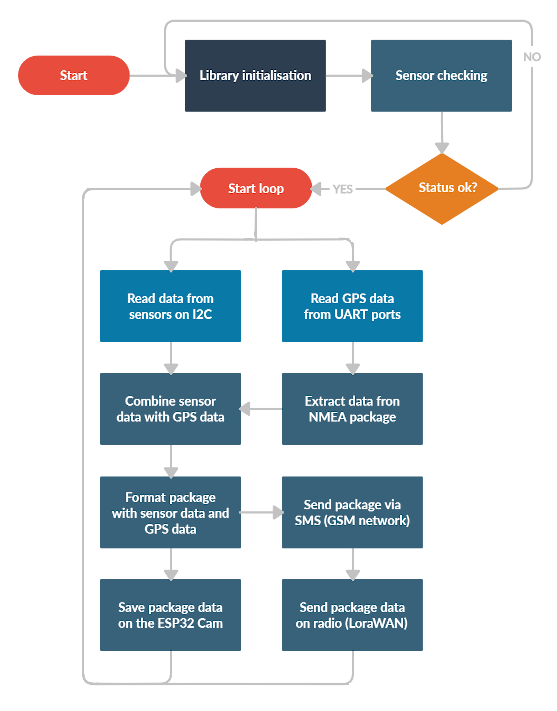
\includegraphics[width=9cm]{Software_diag.png}
    \caption{\small{Software diagram.}}
    \label{fig:codeblocks}
\end{figure}

We will be using Git extensively to keep track of changes to the codebase. This allows us to easily roll back to a previous version if a new feature breaks the code. With Git, we can collaborate on the codebase and track changes made by different team members, ensuring a smooth and efficient development process.

% \begin{wrapfigure}{r}{0.5\textwidth}
%     \centering
%     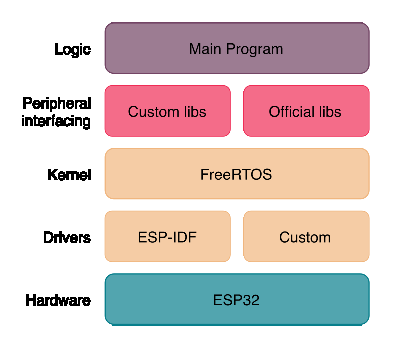
\includegraphics[width=7.5cm]{images/img_Cansat_RTOS.eps}
%     \caption{\small{CanSat software state diagram.}}
%     \label{fig:rtos}
% \end{wrapfigure}


Additionally, we are planning to develop a custom software application that will run on the ground station. This application will receive the telemetry data from the payload and interpret it, visualizing the information on real-time graphs. The software will extract sensor data such as acceleration, GPS coordinates, pressure, and more from the raw data packets, allowing us to monitor the payload's performance and the environmental conditions it encounters. The software will also log the data to ensure that no valuable measurements are lost. 